\documentclass[11pt]{article}

\usepackage{natbib}
\usepackage{setspace}
\usepackage[left=2.5cm,top=2.8cm,right=2.5cm,bottom=2.8cm]{geometry}
\usepackage{graphicx}
\usepackage{amsmath,amssymb}
\usepackage{amsmath}
\usepackage{theorem}
\usepackage{version}
\usepackage{multirow}
\usepackage{listings}
\usepackage{mathtools}
\usepackage{hyperref}
\usepackage{algpseudocode}
\usepackage{amssymb}
\usepackage{tikz}
\usepackage{algorithm}
\usepackage{algorithmic}
\usepackage{minted}
\usepackage{graphicx}
\usepackage{tikz}
\newcommand{\circo}{~\raisebox{1pt}{\tikz \draw[line width=0.6pt] circle(1.1pt);}~}
\usetikzlibrary{arrows,arrows.meta,decorations,decorations.pathreplacing,calc,matrix}

\definecolor{Red}{rgb}{1,0,0}
\definecolor{Blue}{rgb}{0,0,1}
\definecolor{Green}{rgb}{0,1,0}
\definecolor{magenta}{rgb}{1,0,.6}
\definecolor{lightblue}{rgb}{0,.5,1}
\definecolor{lightpurple}{rgb}{.6,.4,1}
\definecolor{gold}{rgb}{.6,.5,0}
\definecolor{orange}{rgb}{1,0.4,0}
\definecolor{hotpink}{rgb}{1,0,0.5}
\definecolor{newcolor2}{rgb}{.5,.3,.5}
\definecolor{newcolor}{rgb}{0,.3,1}
\definecolor{newcolor3}{rgb}{1,0,.35}
\definecolor{darkgreen1}{rgb}{0, .35, 0}
\definecolor{darkgreen}{rgb}{0, .6, 0}
\definecolor{darkred}{rgb}{.75,0,0}
\definecolor{lightgrey}{rgb}{.7,.7,.7}

\definecolor{clemson-orange}{RGB}{234,106,32}
\definecolor{chicago-maroon}{RGB}{128,0,0}
\definecolor{northwestern-purple}{RGB}{82,0,99}
\definecolor{cornell-red}{RGB}{179,27,27}
\definecolor{sauder-green}{RGB}{171,180,0}
%\definecolor{gray}{RGB}{192,192,192}
\definecolor{lawngreen}{RGB}{0,250,154}

\setcounter{MaxMatrixCols}{10}

\onehalfspacing
\newtheorem{theorem}{Theorem}
\newtheorem{acknowledgement}{Acknowledgement}
\newtheorem{algorithm}{Algorithm}
\newtheorem{assumption}{Assumption}
\newtheorem{axiom}{Axiom}
\newtheorem{case}{Case}
\newtheorem{claim}{Claim}
\newtheorem{conclusion}{Conclusion}
\newtheorem{condition}{Condition}
\newtheorem{conjecture}{Conjecture}
\newtheorem{corollary}{Corollary}
\newtheorem{criterion}{Criterion}
\newtheorem{definition}{Definition}
\newtheorem{example}{Example}
\newtheorem{exercise}{Exercise}
\newtheorem{lemma}{Lemma}
\newtheorem{notation}{Notation}
\newtheorem{problem}{Problem}
\newtheorem{proposition}{Proposition}
{\theorembodyfont{\normalfont}
\newtheorem{remark}{Remark}
}
\newtheorem{summary}{Summary}
\newenvironment{proof}[1][Proof]{\textbf{#1.} }{\hfill \rule{0.5em}{0.5em} \bigskip}
\newenvironment{soln}[1][Soln]{\textbf{#1:} }{\hfill \rule{0.5em}{0.5em}}
\renewcommand{\cite}{\citeasnoun}
\renewcommand{\theenumii}{(\alph{enumii})}
\renewcommand{\labelenumii}{\theenumii}
\renewcommand{\theenumiii}{\roman{enumiii}}
\renewcommand{\labelenumiii}{\theenumiii.}

\usepackage[nameinlink]{cleveref}
\crefname{assumption}{Assumption}{Assumptions}
\crefname{lemma}{Lemma}{Lemmas}
\crefname{theorem}{Theorem}{Theorems}
\crefname{corollary}{Corollary}{Corollaries}
\crefname{proposition}{Proposition}{Propositions}
\crefname{claim}{Claim}{Claims}
\crefname{procedure}{Procedure}{Procedures}
\crefname{algorithm}{Algorithm}{Algorithms}
\crefname{figure}{Figure}{Figures}
\crefname{remark}{Remark}{Remarks}
\crefname{section}{Section}{Sections}
\crefname{procedure}{Procedure}{Procedures}
\crefname{example}{Example}{Examples}
\crefname{definition}{Definition}{Definitions}
\crefname{table}{Table}{Tables}
\crefname{align}{}{}
\crefname{enumi}{}{}
\crefname{conjecture}{Conjecture}{Conjectures}
\crefname{step}{Step}{Steps}
\crefname{appendix}{Appendix}{Appendices}
\crefname{footnote}{Footnote}{Footnotes}

\begin{document}


\begin{center}
    \textbf{CS 326 - Analysis of Algorithms - HW 5}\\
\end{center}


\begin{flushleft}
    \textit{Prof. M. Grigni\hfill11/18/2022 \hfill Hridansh Saraogi} \\
    \vspace{0.15cm}
    \small {Help taken from: Prof. Grigni, and Zhenke Liu}\\
    \small {Collaborators: Rhea Ramchandran}
\end{flushleft}


\begin{enumerate}

\item Problem 1 (push-relabel bipartite matching). \\
Suppose we want to find a maximum matching in a bipartite graph G. We first construct the flow network G' as described in Section 26.3, and then we use the generic push-relabel algorithm of Section 26.4 (instead of Ford-Fulkerson). Argue that this approach runs in O(VE) time.  Hint: show every push is saturating.
    \begin{enumerate}
        \item Flow network: a directed graph where each edge has both a capacity and it receives a flow
        \item The edge capacity for an edge (u, v) is e(u, v) = 1\\
        This gives us that the flow: $0 \leq f(u,v) \leq 1$
        \item The push-relabel algorithm of Section 26.4 uses integer capacities\\$\therefore$ the overflow u and the preflow f will always have integer values
        \item Based on this principle, the pushes will always be saturating and none of them will be non-saturating.\\
        Since we know how to implement 'relabel' in O(1) time and 'push' in O(1) time as well, it is will be helpful for this question.
        \item There will be O(VE) saturating 'Push'es and O($V^2$) Relabels
        \item Based on this, we can conclude that the total time will be O(VE)\\
        Computed as O(VE + $V^2$) = O(VE)  $->$ since E is bigger than V
    \end{enumerate}

\pagebreak

\item Problem 2 (push-relabel gap heuristic). Exercise 26.5-5, page 760.\\
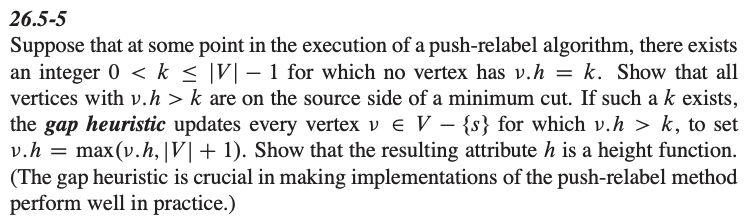
\includegraphics[scale=1]{HW5_Q2.png}
    \begin{enumerate}
        \item Some initializations: Let h(v) = vh $-> $this is a height function\\
        Let k hold a value with the following bounds: $0 < k < \|V\|$
        \item Let us assume that when h(v) = k, there is no such v which belongs to V (a vertex v which belongs to a set of vertices V)
        \item We will set up the height function's h'(v) as a piecewise function, with values depending on the value of k \\
        \begin{equation}
            h'(v)=
                \begin{cases}
                    $\mid V \mid$ & \text{if } v=s\\
                    h(v) & \text{if } h(v)<k\\
                    max(h(v), \mid V \mid +1) & \text{if } h(v) > k 
                \end{cases}
        \end{equation}
        \item Goal: to confirm that the above piecewise function is an appropriate function for modeling the height of the preflow f. Since the max() function is introduced by the gap heuristic, we need to prove that it exists\\
    \end{enumerate}
    \begin{enumerate}
        \item Facts: h' is an integer\\h'(s) = $\mid V \mid$\\ h'(t) = 0
        \item Given that a vertex (u, v) belongs to the Gap Heuristic, we know the following:\\
        $h(u) \leq h(v) + 1$\\
        Using the above known, we need to show that using the piecewise function, \\$h'(u) \leq h'(v) + 1$
        \item Let us consider each of the pieces of the h'(v) function:
        \begin{enumerate}
            \item Piece 1: when v=s\\
            h'(v) = $\mid V \mid$\\
            This gives: $h(u) \leq \mid V \mid + 1 \hspace{0.5cm} \rightarrow \hspace{0.5cm} h'(u) \leq \mid V \mid + 1 \hspace{0.5cm} \rightarrow \hspace{0.5cm}  h'(u) = h'(v) + 1$
            
            \item Piece 2: when $h(v)<k$\\
            Since h(u) != k, h(u)$<$k\\
            $\therefore h'(u) = h(u)$. Hence $h'(v) = h(v)$
            
            
            \item Piece 3: when $h(v)>k$\\
            $h'(v) = max(\mid V \mid + 1, h(v))$\\
            $h'(u) \leq max(\mid V \mid + 1, h(u))$\\
            $h'(u) \leq max(\mid V \mid + 1, h(v)+1)$\\
            $h'(u) \leq max(\mid V \mid + 1, h(v))+1$\\
            $h'(u) = h(u)+1$\\
            Hence proved
        \end{enumerate}
        \item Since the Gap Heuristic does not employ any edges from sink S to another, R (every vertex is of the form $h(v) < k$). Using this, one can conclude that the heights of labels can be raised in sink S
        
        \item Given the way that S and R are set up, the gap heuristic does not permit them to map to each other. For example, a vertex from S cannot be connected to a vertex on R because there is not an edge which goes from S to R
        \item The above is a result of the fact that a minimal cut corresponds to disconnected parts of the residual graph for a max flow.
        \item The above does not necessitate that it is a min-cut of the Gap Heuristic - this is explained in the textbook
        \item Proof by Contradiction, for a min-cut where the vertex which had the gap heuristic is on the cut's sink-side.
        \begin{enumerate}
            \item For such a min-cut, the residual flow network needs to be considered.
            \item This network will be saturated 
            \item 
        \end{enumerate}
        \item Hence we see that it is not a minimum cut - because it has capacity of 2.\\
        To be a min-cut, it would have had to have capacity of 1
    \end{enumerate}
    
\pagebreak

\item Problem 3(HAM-CYCLE listing). Exercise 34.2-3, page 1065.\\
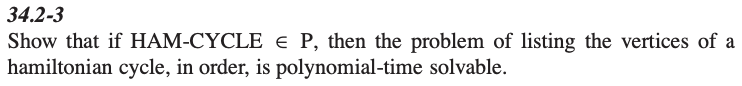
\includegraphics[scale=1]{HW5_Q3.png}
    \begin{enumerate}
        \item Hamiltonian signifies that it consists of a Hamilton cycle\\
        Given that the HAM-CYCLE belongs to P, let us assume that it is solvable in polynomial-time, and therefore contains a Hamiltonian cycle.
        \item Let us now pick one vertex v in the graph, it could be any vertex\\
        Then let us look at the set of edges that correspond to a certain vertex v, we will eliminate all edges, except two of that vertex.
        \item We will continue this method through all the pairs of edges, until the duo which forms a hamiltonian graph is found.
        \item When looking at all pairs, since a vertex's degree is restricted by one less than the number of vertices, we are actually just squaring this number. Essentially: n-1 belongs to $O(n^2)$\\
        This signifies that the runtime is polynomial since we are running the testing-method polynomial number of times.
        \item Upon testing v's adjacent vertices, and continuing the elimination process, till only $\|V\|$ (abs. value, v belongs to V) edges are left, we arrive upon a hamiltonian circuit which was developed through our process described above.
        \item Many search algorithms can then be run on this hamiltonian cycle to obtain the order of vertices. \\
        
        \textit{Note: }Repeating the process, and looking at v's adjacent vertices was essentially considering the hamiltonicity of each vertex.
    \end{enumerate}

\pagebreak

\item Problem 4 ($\leq P$ is transitive). Exercise 34.3-2, page 1077. \\Hint: if p(n) and q(n) are polynomials, then so is p(q(n)).\\
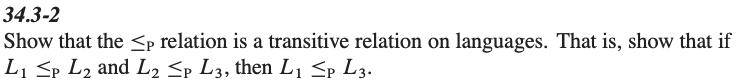
\includegraphics[scale=1]{HW5_Q4.png}
    \begin{enumerate}
        \item Showing that the $\leq_p$ relation is transitive on languages:\\
        Let us begin by assuming that the first inequality is true ($L_1 \leq_p L_2$), and that a function $f_1$ is a polynomial time reduction function.
        \item This function follows that only if $f_1(x)$ belongs to $L_2$,  x belongs to $L_1$
        \item Looking at the rest of the relations given in the question, the above methodology tell us:\\
        For $L_2 \leq_p L_3$: function $f_2$ is the polynomial time reduction function; only if $f_2(x)$ belongs to $L_3$,  x belongs to $L_2$
        \item Using this comprehension, we can:
            \begin{enumerate}
                \item $f_2$\circo $f_1$  can be calculate in polynomial time
                \item x will belong to $L_2$ if and only if $f_2(x)$ belongs to $L_3$
            \end{enumerate}
        \item Given all the above, one can conclude that $\leq_p$ is a transitive relation because $L_1 \leq_p L_3$\\
    \end{enumerate}
    \begin{enumerate}
        \item Another point to consider:\\
        How long does it take to compute f2(f1(x))?
        \begin{enumerate}
            \item Problem: the length of f1(x) could be much longer than $n=\|x\|$
            \item Solution: showing that the total time is still bounded by a polynomial\\
            Since both $f_1(x)$ and $f_2(x)$ are polynomials, and $f_1(x)$ belongs to $L_2$ and $f_2(x)$ belongs to $L_3$, then:\\
            we observe that x belongs to $L_1$ and f2(f1(x)) belongs to $L_3$
            \item $\therefore L_1 \leq_p L_3$ and we can say that f2(f1(x)) is also calculatable in polynomial time
            
            
        \end{enumerate}
    \end{enumerate}

\pagebreak
\item Problem 5\\
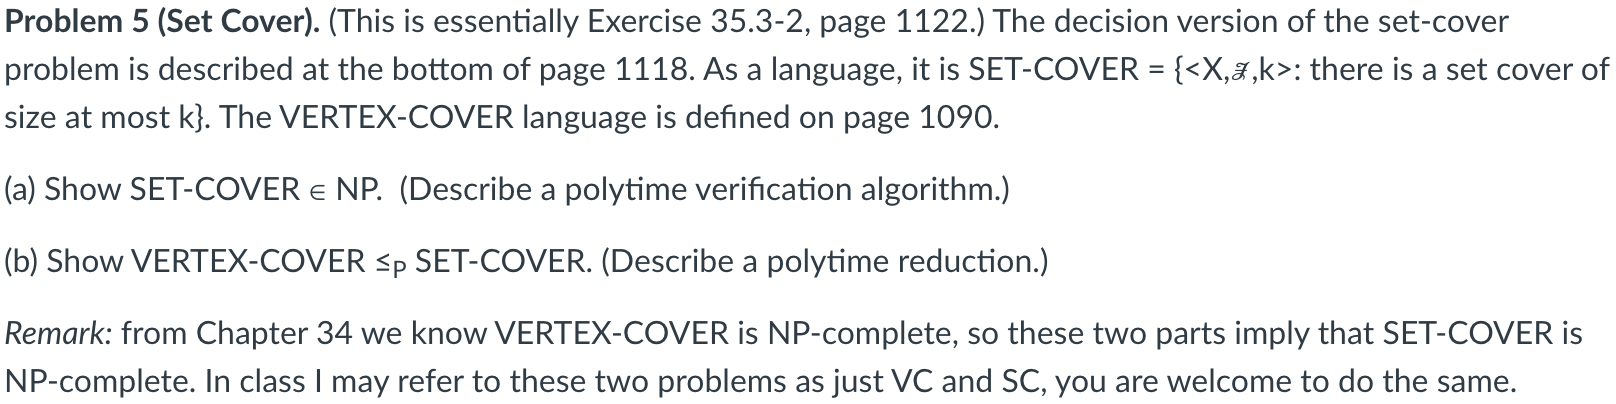
\includegraphics[scale=0.55]{HW5_Q5_1.png}\\
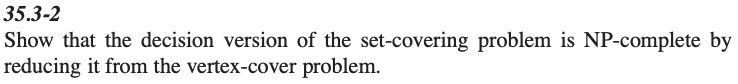
\includegraphics[scale=1]{HW5_Q5_2.png}
    \begin{enumerate}
        \item Solution to Ex 35.3-2:
        \begin{enumerate}
            \item Things needed in polynomial time:
        \begin{enumerate}
            \item X's each element is minimum in one of the sets
            \item The number of sets doesn’t exceed k.
        \end{enumerate}
        \item If both of these are met, the set-covering will be in NP
        \item Given the above, it is now needed to show that it is NP-hard. \\Method: reduce from the vertex-cover problem
        \begin{enumerate}
            \item Let us work on a graph G = (V, E)\\
            We will have a set of vertices V' which are all vertices from G with degree 0
            \item Let's now create a set S which comprises of each vertex in V, and all of its neighbours
            \item Due to this, S will be a proper subset of V
            \item We will also introduce another set C which contains all elements of S, where each element belongs to set V'
            \item If S is a vertex of cover of G (which it will be if S is a proper subset) and has a maximum of k vertices, then $\{S_v|v$ belongs to S and V'\}. Based on this, V' will be considered a set cover having a maximum of k vertices as well.
            \item Let us consider the case where the set cover for G (following the maximum of k vertices) does not exist, we would try to find another set cover. One such set cover would be for V' which would encompass no more than k sets from the set mentioned above $->$ \{$S_v|v$ belongs to V'\}
            \item Based on this, a contradiction can be developed: what if an element is used which belongs to the new set cover and will be considered the K-th element to fulfill the vertex cover G.
            \item Using the above, G will get its K-th element for its vertex cover. Although, if V' did not have a K-th element, this would not be possible
            \item $\therefore$ we can conclude that set covering is NP-hard, and it will be NP-complete.
            \\
            \textit{Clarification: }It is unknown whether G has a vertex cover of size k; we see that the input is in VC if and only if the output is in SC.
        \end{enumerate}
        \end{enumerate}
        
        \item More explicitly, the SET-COVER belongs to NP since:
        \begin{enumerate}
            \item Certificate for the problem: list of subsets of size k, required for set-cover
            \item Check that each element occurs at least once in the subsets
            \item Takes polynomial time, hence SC belongs to NP
            \item It is a "verifier algorithm" (with input x, or $<X,F,k>$)
        \end{enumerate}
        
        \item VERTEX-COVER $\leq_p$ SET-COVER because:
        \begin{enumerate}
            \item Showing that SC is NP hard:
            \begin{enumerate}
                \item Reduce VC to SC
                \item $\{S_v|v$ belongs to V'\}
                \item VC of k vertices formed...formed by each edge connecting to 1 vertex at minimum
                \item For k vertices, $S_v$ contains all edges connected to vertex v. Given this, a SC of size k is formed
                \item Contradiction explained in G.
            \end{enumerate}
            \item Hence we see that the input is in VC if and only if the output is in SC.
            \item It is  a "reduction algorithm" (with input $<G,k>$, output $<X,F,k'>$)
        \end{enumerate}
        \item Given that we saw it meets the required criteria, it is NP-Complete (and NP-hard)
    \end{enumerate}
    
\end{enumerate}
\pagebreak


\end{document}

